\documentclass[aps,prd,onecolumn,nofootinbib,superscriptaddress]{revtex4-2}

\usepackage[utf8]{inputenc}
\usepackage[T1]{fontenc}
\usepackage{lmodern}
\usepackage{amsmath,amssymb,amsfonts,bm}
\usepackage{graphicx}
\usepackage{xcolor}
\usepackage{hyperref}
\usepackage{siunitx}
\usepackage{enumitem}
\usepackage{booktabs}

\hypersetup{colorlinks=true,linkcolor=blue,citecolor=blue,urlcolor=blue}

\newcommand{\dd}{\mathrm{d}}
\newcommand{\trm}{\mathrm}

\begin{document}

\title{TCV-$\phi$ VIII: toward a one-scalar completion\\
from cohesive-vacuum topology and coherent-sector $\Phi_2$ emergence}

\author{Cyrille LECROQ}
\affiliation{Independent Researcher}

\date{\today}

\begin{abstract}
This paper investigates whether the ultralight $\Phi_2$ sector of the canonical TCV-$\phi$ programme can be reinterpreted as an emergent collective mode of the CC-$\Phi_1$ cohesive microstructure.
The study is organized as a reproducible inverse/direct pipeline:
PMNS-like flavour constraints are first translated into modal and topological requirements, candidate cluster geometries are then compared under common diagnostics, and the leading candidates are finally tested against $\Phi_2$ emergence, reduced homogeneous ULDM-like evolution, and microscopic closure criteria.
The main result is structural rather than theorem-level:
closed twisted topologies are consistently favored over rigid or open cluster toys, and the twisted-multi-ring geometry gives the strongest combined PMNS + $\Phi_2$ bridge signal.
For the full twisted-multi-ring bridge we obtain a calibrated emergent mass $m_2 \simeq 8.98\times10^{-23}\,\mathrm{eV}$, joint and robustness pass fractions close to unity and $0.72$ respectively, and a reduced homogeneous evolution compatible with $\rho\propto a^{-3}$.
Dedicated micro-closure tests remain partial at the operator level, but residual diagnostics show that the failure is dominated by omitted higher internal modes rather than by inter-ring topology itself.
When the reduction is restricted to a coherent global sector, the effective closure improves significantly, which motivates the interpretation of $\Phi_2$ as a coherent-sector effective mode of CC-$\Phi_1$ rather than as a full microscopic closure of the entire microstructure.
The present status is therefore a structured one-field route with strong topology-sensitive support and a sector-restricted effective closure, while strict global micro-closure remains open.
\end{abstract}

\maketitle

\section{Introduction}
Papers~I--VII established the canonical two-scalar EFT layer of TCV-$\phi$ and its main phenomenological sectors:
background evolution, perturbations, compact objects, and Planck confrontation.
The remaining conceptual question is whether $\Phi_2$ must remain a separate effective scalar, or whether it can instead emerge as a collective low-energy mode of the CC-$\Phi_1$ cohesive microstructure.

This paper is written in a deliberately conservative spirit.
It does not claim a final microscopic proof.
Instead, it organizes the one-field question into a reproducible programme with explicit diagnostics, stop rules, and control geometries.
Its status is that of a structured one-field benchmark paper rather than a final closure theorem.

\section{Scope and methodological status}
The workflow adopted here has four stages:
\begin{enumerate}[label=\arabic*)]
  \item infer modal and geometric requirements from PMNS-like flavour structure;
  \item compare geometry families under common PMNS and structure scores;
  \item test whether the same leading geometries support an emergent $\Phi_2$ mode;
  \item evaluate partial microscopic closure and one-field consistency.
\end{enumerate}
All results quoted below are script-backed and archived in the Paper-08 workspace.
We distinguish throughout between:
\begin{itemize}
  \item exact linear-algebra diagnostics;
  \item heuristic effective-field reductions;
  \item exploratory micro-closure attempts.
\end{itemize}
When a result is obtained from a simplified bridge or family-level screening stage, it is explicitly labelled as such; the strongest claims in this paper are reserved for the dedicated twisted-multi-ring PMNS, full-bridge, residual-diagnostic, and dedicated micro-closure layers.

\section{Inverse/direct geometry programme}
The first step is an inverse PMNS analysis:
starting from large $\theta_{23}$, small but non-zero $\theta_{13}$, and moderate $\theta_{12}$, we infer a preferred modal structure with
\begin{itemize}
  \item a quasi-degenerate doublet,
  \item a singlet+doublet split,
  \item weak singlet-doublet mixing,
  \item controlled symmetry breaking,
  \item and a preference for closed non-trivial topology.
\end{itemize}
These inferred constraints are then used to rank explicit geometry families.

\begin{figure}[t]
  \centering
  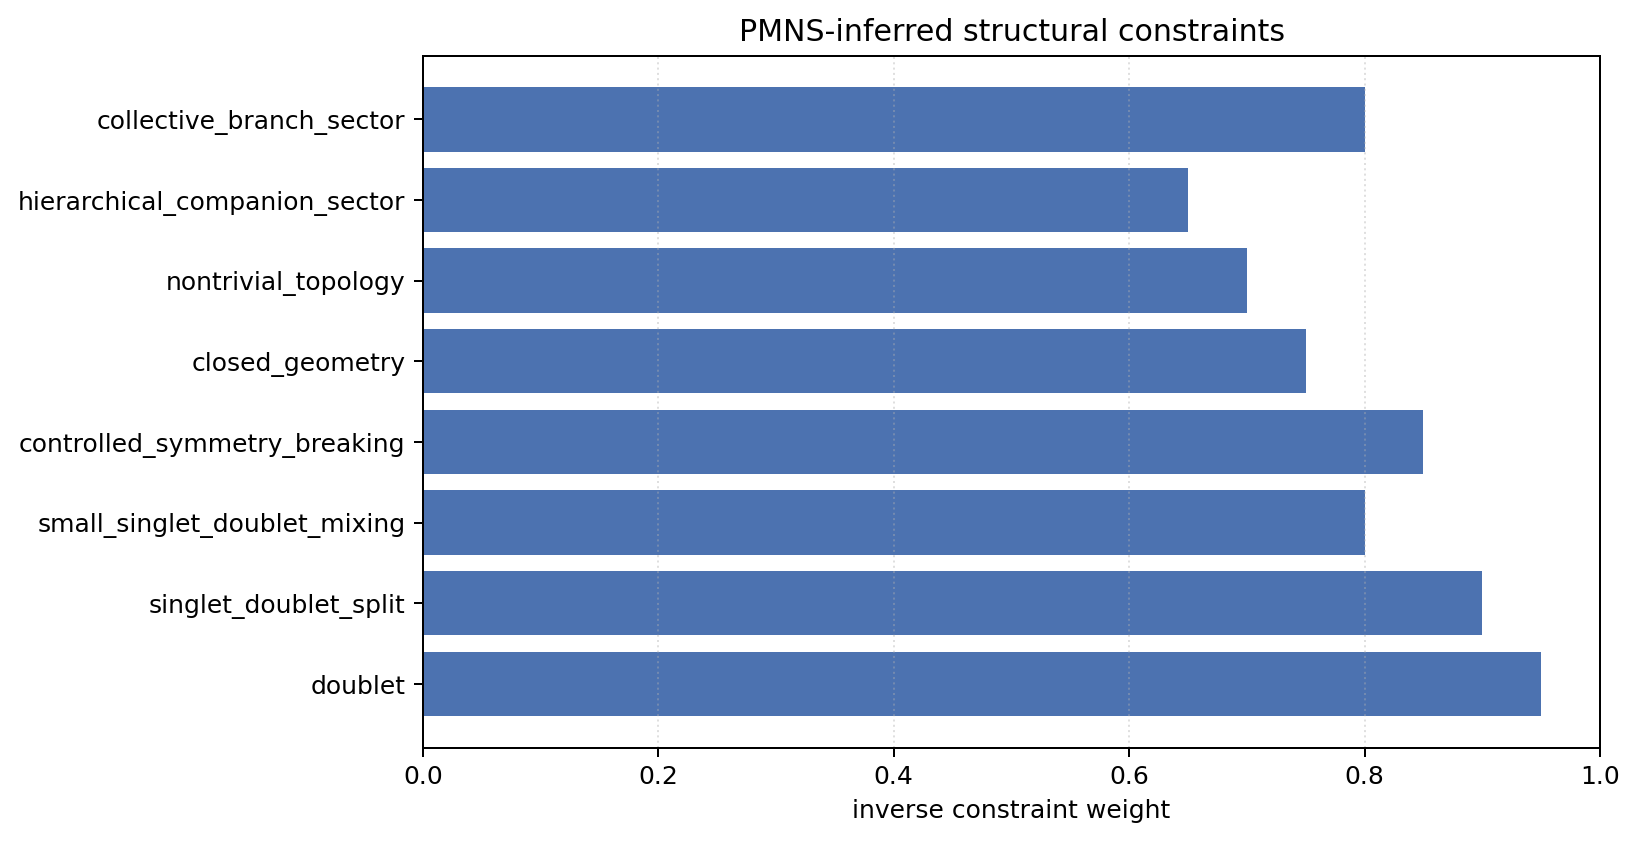
\includegraphics[width=0.80\textwidth]{../figs/pmns_inverse_constraints.png}
  \caption{Inverse PMNS constraint profile used to guide the geometry scan.}
  \label{fig:paper8-inverse-constraints}
\end{figure}

\begin{figure}[t]
  \centering
  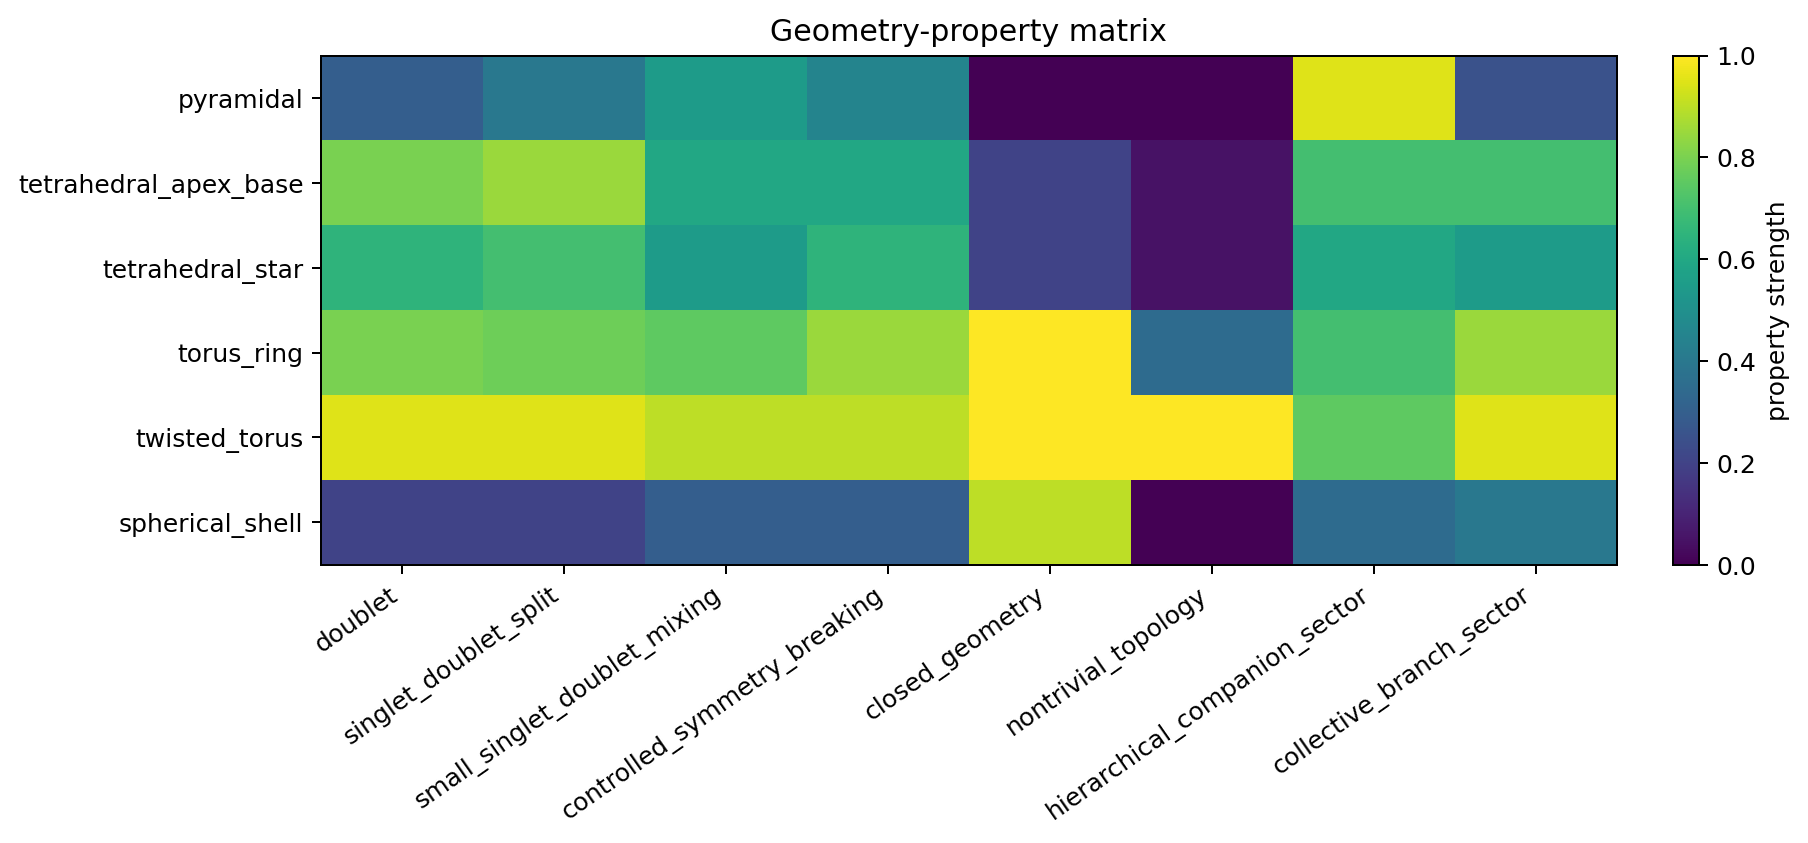
\includegraphics[width=0.88\textwidth]{../figs/pmns_geometry_property_matrix.png}
  \caption{Geometry-property matrix for the inverse/direct scan. Closed twisted topologies satisfy the largest subset of inferred constraints.}
  \label{fig:paper8-geometry-matrix}
\end{figure}

The resulting family-level rankings show that rigid geometries remain disfavored, while twisted closed topologies dominate both PMNS and bridge-oriented structural scores.
This is the point where geometry becomes a dynamical ingredient rather than a decorative model choice.
At this stage, however, the rankings should still be read as family-selection diagnostics rather than as candidate-level proofs.

\section{From twisted torus to twisted multi ring}
The historical turning point of the programme was the twisted-torus cluster.
It was the first explicit geometry to produce a coherent joint signal for PMNS-like flavour and emergent-mode diagnostics.
However, the same systematic scan that validated the topological direction also suggested that the twisted torus is not the endpoint of that family.

Two candidate extensions were tested at the same broad topological level:
phase-loop and twisted-multi-ring.
The phase-loop proxy looked promising but failed to maintain its performance when promoted to a dedicated flavour toy.
By contrast, twisted-multi-ring remained strong under dedicated PMNS tests and therefore became the main candidate.

\begin{table}[t]
  \centering
  \begin{tabular}{lcc}
    \toprule
    Candidate & $S_{\rm PMNS}$ & Strict fraction within natural scan \\
    \midrule
    Twisted torus & 0.519 & 0.0194 \\
    Twisted multi ring & 0.235 & 0.0415 \\
    \bottomrule
  \end{tabular}
  \caption{Dedicated PMNS-level comparison within the leading twisted-topology family.}
  \label{tab:paper8-twisted-headtohead}
\end{table}

\begin{figure}[t]
  \centering
  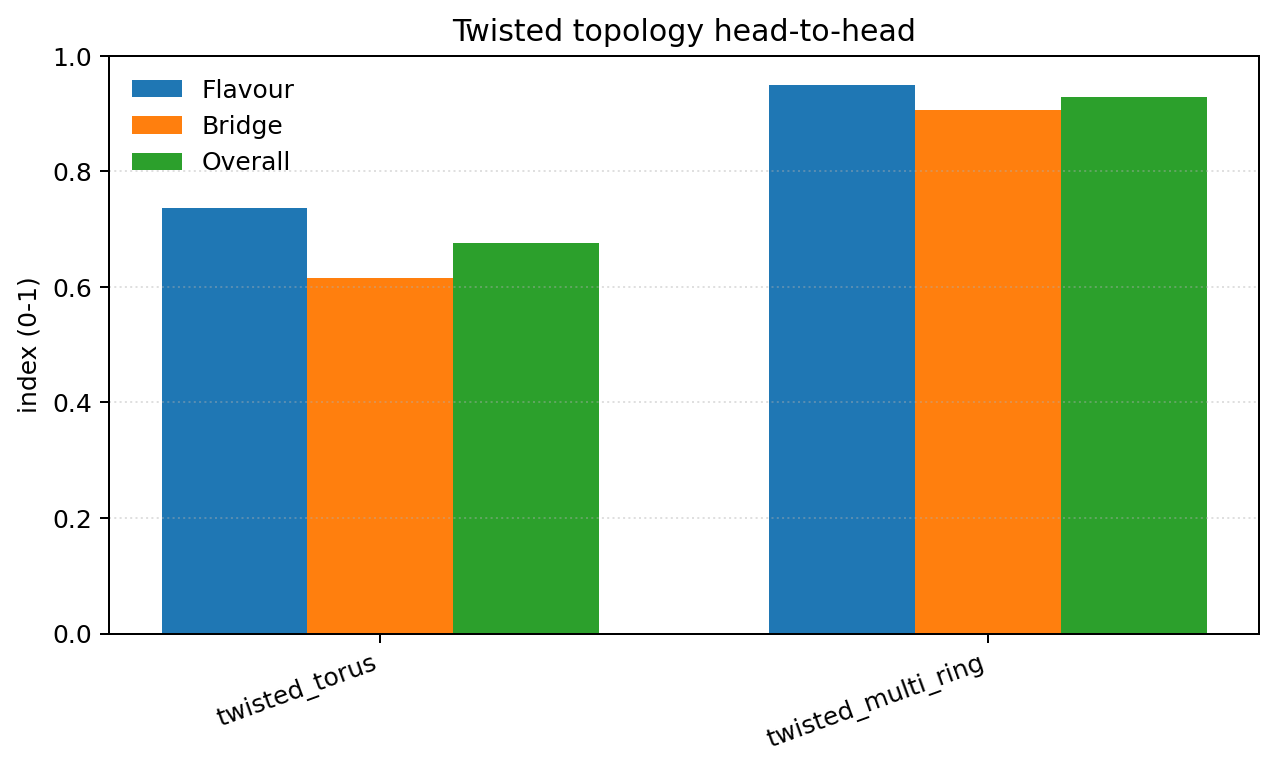
\includegraphics[width=0.84\textwidth]{../figs/twisted_topology_headtohead.png}
  \caption{Head-to-head comparison between the historical twisted-torus benchmark and the current twisted-multi-ring candidate.}
  \label{fig:paper8-headtohead}
\end{figure}

The gain is not limited to a single benchmark point.
For the twisted-multi-ring sector-compatibility run, the strict lepton robustness fraction reaches
\begin{equation}
f_{\rm strict}^{(\ell)} \simeq 0.874,
\end{equation}
while the quark-like toy remains weakly mixed.
This supports the interpretation that twisted-multi-ring is not merely a numerically lucky refinement, but a stronger geometry in the same closed twisted family.
The role of twisted torus in this paper is therefore historical and methodological, while the role of twisted-multi-ring is candidate-level and prospective.

\section{Emergent $\Phi_2$ from the twisted topology family}
The central question is whether the same geometry that improves flavour also supports a viable emergent $\Phi_2$ mode.
For this reason, the leading geometries are passed through a dedicated emergence pipeline evaluating:
\begin{itemize}
  \item light-mode softness and collectiveness,
  \item effective mass calibration,
  \item canonical capture and topology-aware source overlap,
  \item reduced homogeneous ULDM-like evolution,
  \item and size scaling.
\end{itemize}
In the present bridge layer, the quoted physical mass is obtained from a calibrated proxy.
More precisely, the dimensionless light-mode quantity $m_{2,{\rm proxy}}$ is mapped to physical units through the same reference normalization used in the family-level bridge stage, with a ULDM anchor scale of $10^{-22}\,\mathrm{eV}$.
The relevant quantity for interpretation is therefore not only the absolute calibrated value, but also the logarithmic deviation from the canonical ULDM window.

At the family level, the twisted-torus benchmark already showed that topology matters.
At the dedicated-candidate level, twisted-multi-ring is stronger.

\begin{figure}[t]
  \centering
  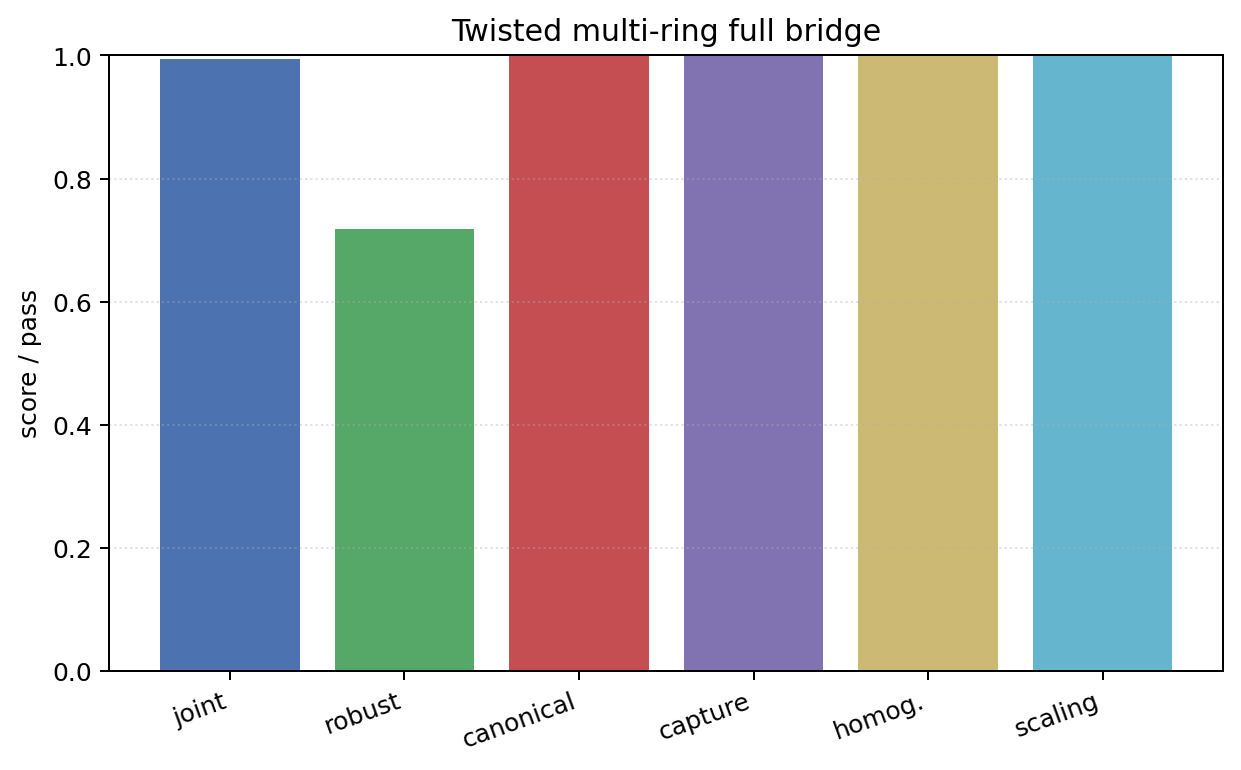
\includegraphics[width=0.86\textwidth]{../figs/twisted_multi_ring_full_bridge_dashboard.png}
  \caption{Full twisted-multi-ring bridge diagnostics.}
  \label{fig:paper8-full-bridge}
\end{figure}

For the full twisted-multi-ring bridge we obtain
\begin{equation}
f_{\rm joint}\simeq 0.994,\qquad
f_{\rm robust}\simeq 0.718,\qquad
m_2 \simeq 8.98\times10^{-23}\,\mathrm{eV},
\end{equation}
with all current bridge checks passing, including canonical normalization, topology-aware mode capture, homogeneous evolution, and size-scaling consistency.
Here $f_{\rm robust}$ denotes the fraction of disorder-perturbed realizations that continue to satisfy the combined softness, gap, and collectiveness conditions used in the bridge diagnostics.
The best-fit reduced homogeneous evolution gives
\begin{equation}
\frac{\dd \log\rho}{\dd \log a}\simeq -3.0001,
\end{equation}
consistent with the expected ULDM-like regime at late times.
The calibrated mass lies only $|\log_{10}(m_2/10^{-22}\,\mathrm{eV})|\simeq 0.047$ decades away from the canonical ULDM target.
An additional feature of the size-scaling scan is a sharp threshold:
the joint fraction is zero for $N_{\rm total}=48$ and $72$, but rises to $\simeq 0.99$ at $N_{\rm total}=96$ and remains near unity above that scale.
At the present stage we interpret this as evidence for a minimum-size requirement of the twisted-multi-ring topology to sustain coherent light-mode emergence, rather than as a proof of a true phase transition.
This does not yet prove that $\Phi_2$ is fully derived from first principles, but it shows that the one-field route survives a substantially stronger internal bridge test than the earlier family-level proxy stages.

\begin{table}[t]
  \centering
  \begin{tabular}{lcc}
    \toprule
    Metric & Twisted torus & Twisted multi ring \\
    \midrule
    Flavour index & 0.736 & 0.949 \\
    Bridge index & 0.615 & 0.906 \\
    Overall index & 0.675 & 0.928 \\
    \bottomrule
  \end{tabular}
  \caption{Consolidated twisted-topology comparison from \texttt{twisted\_topology\_consolidated\_summary.json}.}
  \label{tab:paper8-consolidated}
\end{table}

\begin{figure}[t]
  \centering
  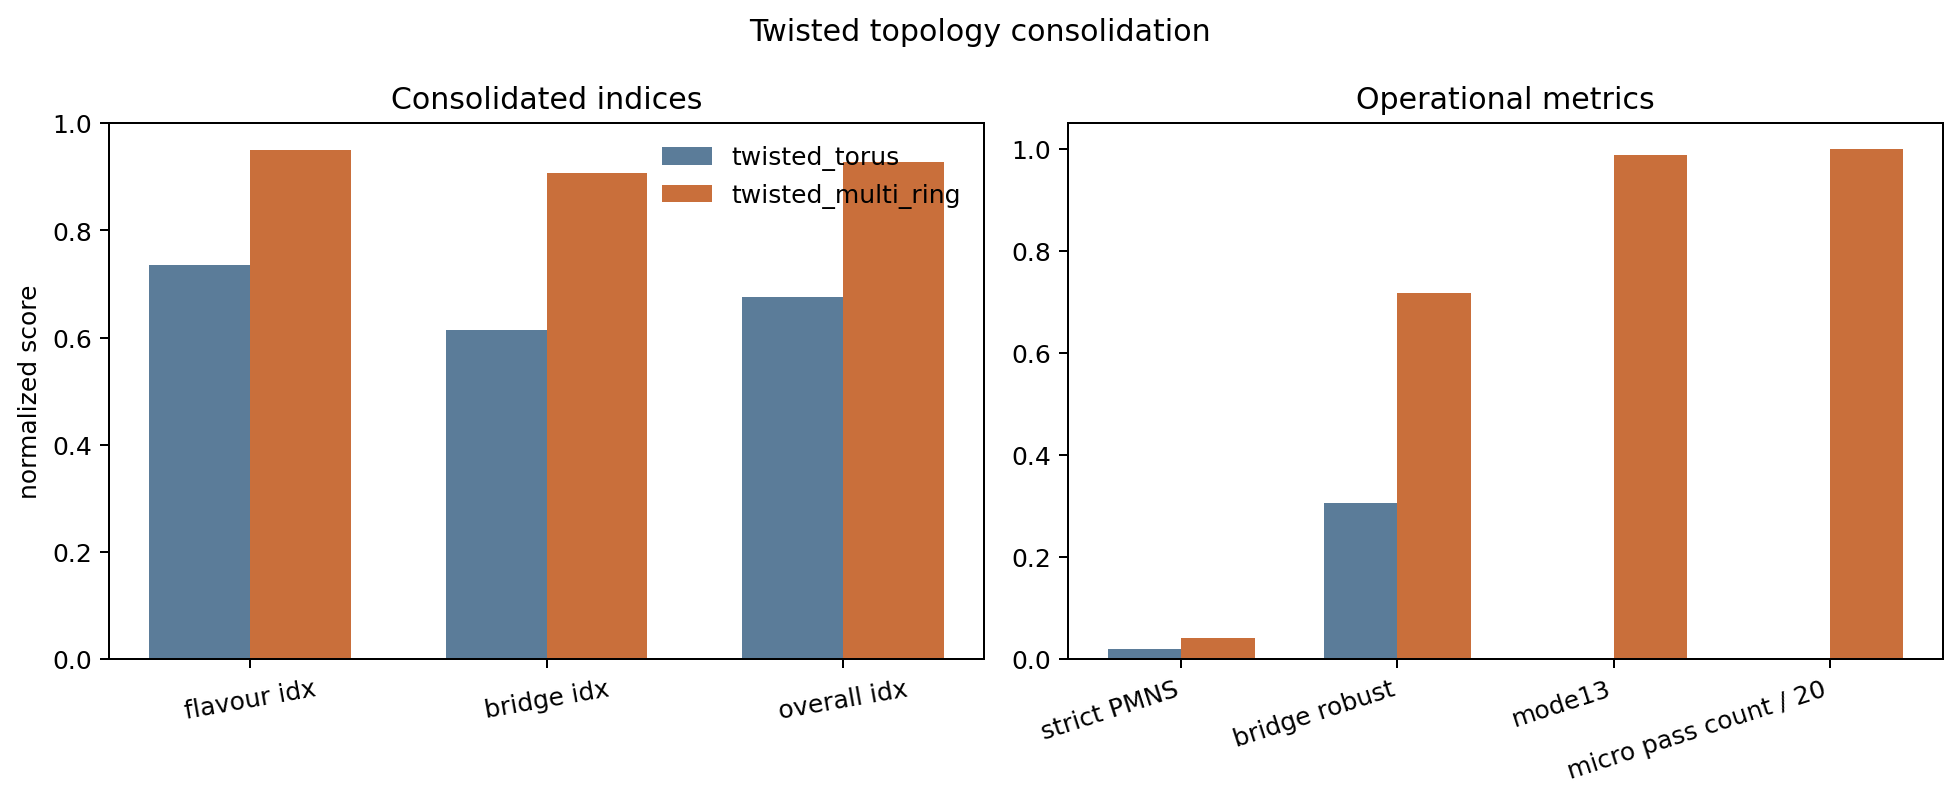
\includegraphics[width=0.86\textwidth]{../figs/twisted_topology_consolidated_dashboard.png}
  \caption{Consolidated dashboard: historical twisted-torus baseline versus current twisted-multi-ring candidate.}
  \label{fig:paper8-consolidated}
\end{figure}

\section{Micro-closure status}
The one-field route would require more than an effective bridge:
it would require a credible microscopic closure showing that the same CC-$\Phi_1$ network can support the effective $\Phi_2$ sector without introducing an independent fundamental scalar.

For the earlier twisted-ring/twisted-torus-like ansatz family, repeated structured extensions eventually hit a stop rule:
the programme remained structurally informative but microscopically incomplete.
This remains an important caution.

The twisted-multi-ring candidate performs better.
Its dedicated micro-closure attempt reaches
\begin{equation}
\texttt{verdict}=\texttt{micro\_closure\_partial\_supported},
\end{equation}
with $20$ passing records on the current grid and a best generalized projection error
\begin{equation}
\epsilon_{13}^{\rm proj}\simeq 2.88\times 10^{-2}.
\end{equation}
This value is the minimum over the dedicated parameter grid explored in the micro-closure scan.
In the present internal convention, ``partial supported'' means that the projection and generalized-diagonalization checks pass reproducibly while the best projection error remains at the few-percent level; a stronger ``full closure'' claim would require this error to be pushed to the percent level or below together with the corresponding microscopic closure conditions.
This is not a theorem-level closure.
It nonetheless moves the one-field interpretation from a vague aspiration to a structured and non-trivial research programme.
This verdict is refined and physically interpreted in Section~\ref{sec:residual} below.

\section{Residual non-closure and effective-sector interpretation}
\label{sec:residual}
The new residual diagnostics clarify why the programme gets close to closure without reaching a full microscopic theorem.
The issue is not primarily the inter-ring coupling topology.
For the twisted-multi-ring benchmark, the retained low-mode projector reproduces the mean source-level projection error
\begin{equation}
\epsilon_{13}^{\rm proj}\simeq 4.51\times 10^{-2},
\end{equation}
but the residual operator norm remains large,
\begin{equation}
\epsilon_{\rm op}^{(n_{\rm keep}=4)} \simeq 0.99996,
\end{equation}
and the omitted spectral fraction is
\begin{equation}
f_{\lambda,{\rm omit}}\simeq 0.9977.
\end{equation}
Here $n_{\rm keep}=4$ should be read against a total mode count $N=96$.
The interpretation is direct:
the low twisted sector already captures the relevant coherent source overlaps, but it does not reconstruct the full microscopic operator because most spectral weight remains in omitted higher internal modes.

The residual block structure points in the same direction.
The dominant residual terms sit on the intra-ring diagonal blocks, at the level of $\sim 0.57$--$0.58$, whereas the inter-ring residual blocks remain only at the level of $\sim 0.028$--$0.029$.
This strongly disfavors the idea that the remaining failure is mainly caused by the topology of inter-ring links.
Instead, the residual is tail-dominated and largely internal to each ring.

The source-bank analysis further sharpens the picture.
Global coherent twist sources such as \texttt{global\_twist\_k1\_sin} and \texttt{global\_twist\_k1\_cos} project almost entirely into the low twisted sector, with low-mode fractions near $0.99$ and $0.98$ respectively.
By contrast, local contrast and twist-pair sources populate the omitted tail very strongly.
This means that the current effective reduction already works for coherent global excitations, but not for the broader set of local or contrastive microscopic excitations.

This interpretation is confirmed by the enlarged-subspace scan.
When the retained space is increased up to $n_{\rm keep}=12$, the coherent-sector mean error drops to
\begin{equation}
\epsilon_{\rm coh}\simeq 8.58\times 10^{-2},
\end{equation}
while local and twist-pair sectors remain much less controlled,
\begin{equation}
\epsilon_{\rm local}\simeq 0.425,
\qquad
\epsilon_{\rm twistpair}\simeq 0.462.
\end{equation}
The corresponding verdict is therefore not full closure but
\begin{equation}
\texttt{verdict}=\texttt{coherent\_sector\_closure\_only}.
\end{equation}

The most conservative reading is then the following:
$\Phi_2$ should not presently be interpreted as a full microscopic image of all CC-$\Phi_1$ excitations.
Rather, it is better interpreted as the effective low-energy mode of a coherent global sector selected within the CC-$\Phi_1$ microstructure.
This is still compatible with the one-field route, but it narrows its mathematical meaning:
the route is presently supported as a coherent-sector EFT closure, not as a closure of the entire micro-operator.

\begin{table}[t]
  \centering
  \scriptsize
  \begin{tabular}{lll}
    \toprule
    Block & Primary artifact & Status label \\
    \midrule
    Inverse PMNS profile & \texttt{pmns\_inverse\_geometry\_constraint\_profile.json} & inverse inference \\
    PMNS/geometry scan & \texttt{pmns\_inverse\_geometry\_scan\_summary.json} & family ranking \\
    Topological extension & \texttt{topological\_geometry\_extension\_summary.json} & extension screening \\
    Twisted head-to-head & \texttt{twisted\_topology\_headtohead\_summary.json} & dedicated comparison \\
    Twisted consolidation & \texttt{twisted\_topology\_consolidated\_summary.json} & consolidated benchmark \\
    Full bridge & \texttt{twisted\_multi\_ring\_full\_bridge\_summary.json} & dedicated bridge \\
    Micro closure & \texttt{twisted\_multi\_ring\_micro\_closure\_full\_summary.json} & partial closure \\
    Residual diagnostic & \texttt{multiring\_residual\_diagnostic\_summary.json} & operator residuals \\
    Effective-sector test & \texttt{multiring\_effective\_sector\_diagnostic\_summary.json} & sector closure \\
    Stop-rule memo & \texttt{phi1\_to\_phi2\_stop\_rule\_and\_position.md} & guardrail \\
    \bottomrule
  \end{tabular}
  \caption{Main script-backed artifacts used in the present Paper-VIII analysis.}
  \label{tab:paper8-status}
\end{table}

\begin{figure}[t]
  \centering
  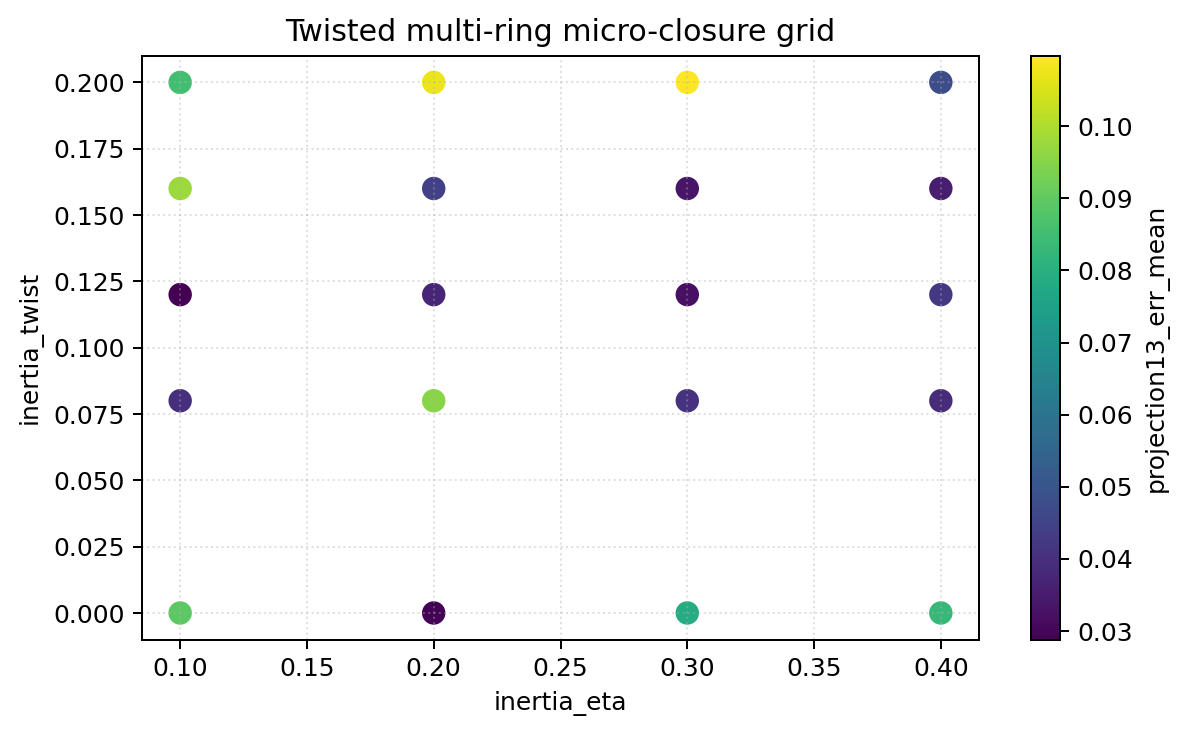
\includegraphics[width=0.84\textwidth]{../figs/twisted_multi_ring_micro_closure_grid.png}
  \caption{Dedicated twisted-multi-ring micro-closure grid. The current status is partial support, not full closure.}
  \label{fig:paper8-micro-grid}
\end{figure}

\section{Interpretation}
The present evidence supports three statements.

First, the geometry of the cohesive vacuum microstructure is not optional in the TCV-$\phi$ framework.
It materially changes both flavour outputs and emergent-mode structure.

Second, the relevant class is no longer just ``non-rigid geometry'' in a loose sense.
The data point more specifically to closed twisted topologies with several coupled channels.

Third, the one-field route is best formulated as:
\begin{center}
CC-$\Phi_1$ microstructure $\longrightarrow$ coherent twisted sector $\longrightarrow$ emergent $\Phi_2$ mode.
\end{center}
This route is strongly supported structurally, but not yet closed microscopically at the full-operator level.
In particular, the data suggest that the relevant ingredient for both flavour and $\Phi_2$ emergence is not a generic deformation, but a specific class of closed twisted multi-channel topologies together with a coherent-sector projection.

\section{Status and conclusion}
The proper current status is:
\begin{itemize}
  \item strong support for topology-sensitive emergence;
  \item strong support for the twisted-multi-ring geometry as the best current joint candidate;
  \item reduced homogeneous ULDM-like consistency;
  \item partial but non-final micro-closure at the full-operator level;
  \item coherent-sector closure support for the effective $\Phi_2$ mode;
  \item no final one-field theorem yet.
\end{itemize}

In that sense, Paper~VIII should not be read as a declaration that the two-scalar EFT is obsolete.
Rather, it defines the strongest current route by which the canonical EFT may admit a deeper one-field completion.
The practical conclusion is therefore conservative:
twisted-torus remains the historical geometry that revealed the correct topological direction, while twisted-multi-ring is now the main candidate on which future one-field and microscopic work should concentrate.
The additional conclusion of the present version is more specific:
the most defensible present interpretation of $\Phi_2$ is that of a coherent-sector effective mode of CC-$\Phi_1$, not that of a complete microscopic closure of all CC-$\Phi_1$ excitations.

\begin{thebibliography}{99}
\bibitem{TCV1} C.~Lecroq, ``TCV-$\phi$ I: an effective cohesive--vacuum field theory and its $\Lambda$CDM-compatible background cosmology,'' preprint (2026), \href{https://doi.org/10.5281/zenodo.19234640}{zenodo.19234640}.
\bibitem{TCV2} C.~Lecroq, ``TCV-$\phi$ II: cohesive bounce, geometric reheating, and baseline baryogenesis/ULDM pipelines,'' preprint (2026), \href{https://doi.org/10.5281/zenodo.19234953}{zenodo.19234953}.
\bibitem{TCV3} C.~Lecroq, ``TCV-$\phi$ III: primordial perturbations across the cohesive bounce and CLASS/CAMB bridge diagnostics,'' preprint (2026), \href{https://doi.org/10.5281/zenodo.19235533}{zenodo.19235533}.
\bibitem{TCV4} C.~Lecroq, ``TCV-$\phi$ IV: cohesive non-singular black holes from static cores to slow rotation in the canonical EFT,'' preprint (2026), \href{https://doi.org/10.5281/zenodo.19235896}{zenodo.19235896}.
\bibitem{TCV5} C.~Lecroq, ``TCV-$\phi$ V: cohesive quantum microstructure from CC-$\Phi_1$ and a controlled bridge to CC-$\Phi_2$ flavour templates,'' preprint (2026), \href{https://doi.org/10.5281/zenodo.19236172}{zenodo.19236172}.
\bibitem{TCV6} C.~Lecroq, ``TCV-$\phi$ VI: critical comparison, risk map, and falsification windows,'' preprint (2026), \href{https://doi.org/10.5281/zenodo.19237306}{zenodo.19237306}.
\bibitem{TCV7} C.~Lecroq, ``TCV-$\phi$ VII: empirical confrontation with Planck likelihoods,'' preprint (2026), \href{https://doi.org/10.5281/zenodo.19237623}{zenodo.19237623}.
\bibitem{NuFIT} I.~Esteban \textit{et al.}, ``NuFIT 5.x global fit of neutrino oscillation parameters,'' online resource (accessed 2026), \url{https://www.nu-fit.org/}.
\end{thebibliography}

\end{document}
